\documentclass{article}
\usepackage{tikz}
\usetikzlibrary{arrows}
\usetikzlibrary[topaths]


\newcount\mycount



\begin{document}

\begin{abstract}
 
Boolean networks have been successfully applied to model gene regulatory networks. Inspired by \cite{Goudarzi} we started to couple boolean with metabolic 
networks to observe their evolution. To do that, we numerically implemented a fixed size population of organisms which divide upon accumulating biomass. 
This is achieved depending on their correct switching of reactions and the consequent production of a target molecule, similar to a percolation in the 
metabolism of that organism. A biomass penalty proportional to the number of enzymes being produced is applied to them, in order to avoid the trivial 
solution (all reactions on).  Each organism has its own boolean network and whenever it divides it produces an exact copy and a mutant one. The food 
molecules in the metabolic network are also present as ingoing nodes in the boolean network, acting thus as sensors of a varying environment. 
Some boolean nodes represent enzymes in the metabolism and turns the corresponding reaction on. This effectively couples both networks of each individual. 
The topology of the metabolic network is shared by all individuals of a population, and different topologies are being proposed as different tasks for the 
populations to solve.

\end{abstract}

The main idea consists of observing how the organisms in a population evolve their gene regulatory structure according to the availability of nutrients. 
To achieve that, we constructed organisms that couple the metabolic network with their boolean network. We couple these two types of networks in the intuitive 
way: whenever a gene $i$ is switched on, if there is a corresponding chemical reaction in which it works as an enzyme it will promote that reaction in case 
the educts are all present within the cell. And to sense the presence of some metabolites we can also send the signal from the metabolic 
network to the boolean network. These nodes in the boolean network that work as sensors are not genes, we will call them sensor nodes.

The boolean network is composed by $G$ genes and $S$ sensor nodes that may have only two states, $\sigma_i \in \{0,1\}$ and a certain interaction topology. 
Every gene or sensor node may potentially repress or enhance other genes, and we define a weight $w_{ij} \in \{-1,0,1\}$ for the efect that gene or sensor node $i$ has on 
gene $j$. This is usually not symmetric. The metabolic network is a bipartite directed network composed by reaction nodes and chemical species nodes. 

The figure below shows a general scheme for one possible instance of an organism.
 
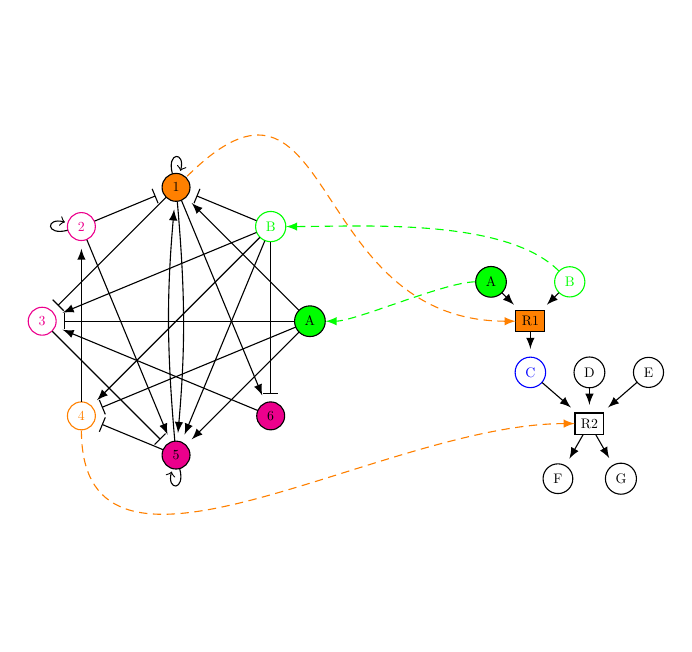
\begin{tikzpicture}[scale=0.5,transform shape]
  
  \node[draw,circle,inner sep=0.15cm,fill=green] (A1) at (0:3.4cm) {A};
  \node[draw,circle,inner sep=0.15cm,green] (B1) at (45:3.4cm) {B};
  \node[draw,circle,inner sep=0.15cm,fill=orange] (1) at (90:3.4cm) {1};
  \node[draw,circle,inner sep=0.15cm, magenta] (2) at (135:3.4cm) {2};
  \node[draw,circle,inner sep=0.15cm, magenta] (3) at (180:3.4cm) {3};
  \node[draw,circle,inner sep=0.15cm, orange] (4) at (225:3.4cm) {4};
  \node[draw,circle,inner sep=0.15cm, fill=magenta] (5) at (270:3.4cm) {5};
  \node[draw,circle,inner sep=0.15cm, fill=magenta] (6) at (315:3.4cm) {6};

  \node[draw,circle,inner sep=0.15cm,fill=green] (A2) at (8cm,1cm) {A};
  \node[draw,circle,inner sep=0.15cm,green] (B2) at (10cm,1cm) {B};
  \node[draw,shape=rectangle,inner sep=0.15cm,fill=orange] (R) at (9cm,0cm) {R1};
  \node[draw,circle,inner sep=0.15cm,blue] (C) at (9cm,-1.3cm) {C};
  \node[draw,circle,inner sep=0.15cm] (D) at (10.5cm,-1.3cm) {D};
  \node[draw,circle,inner sep=0.15cm] (E) at (12cm,-1.3cm) {E};
  \node[draw,shape=rectangle,inner sep=0.15cm] (R2) at (10.5cm,-2.6cm) {R2};
  \node[draw,circle,inner sep=0.15cm] (F) at (9.7cm,-4cm) {F};
  \node[draw,circle,inner sep=0.15cm] (G) at (11.3cm,-4cm) {G};

  \draw[shorten >=0.1cm,-latex] (A2) edge (R);
  \draw[shorten >=0.1cm,-latex] (B2) edge (R);
  \draw[shorten >=0.1cm,-latex] (R) edge (C);
  \draw[shorten >=0.1cm,-latex] (C) edge (R2);
  \draw[shorten >=0.1cm,-latex] (D) edge (R2);
  \draw[shorten >=0.1cm,-latex] (E) edge (R2);
  \draw[shorten >=0.1cm,-latex] (R2) edge (F);
  \draw[shorten >=0.1cm,-latex] (R2) edge (G);



  \path (A2) edge[-latex,green, out=180, in=0,densely dashed,looseness=0.5] (A1)
        (B2) edge[-latex,green, out=135, in=0,densely dashed,looseness=0.7] (B1)
        (R2) edge[latex-,orange, out=180, in=270,densely dashed,looseness=1.0] (4)
        (R) edge[latex-,orange, out=180, in=45,densely dashed,looseness=1.5] (1);

  \draw[shorten >=0.1cm,-latex] (A1) edge (1);
  \draw[shorten >=0.1cm,-|] (A1) edge (3);
  \draw[shorten >=0.1cm,-|] (A1) edge (4);
  \draw[shorten >=0.1cm,-latex] (A1) edge (5);
  \draw[shorten >=0.1cm,-|] (B1) edge (1);
  \draw[shorten >=0.1cm,-latex] (B1) edge (3);
  \draw[shorten >=0.1cm,-latex] (B1) edge (4);
  \draw[shorten >=0.1cm,-latex] (B1) edge (5);
  \draw[shorten >=0.1cm,-|] (B1) edge (6);
  \draw[shorten >=0.1cm,-latex] (1) edge [loop above] (1);
  \draw[shorten >=0.1cm,-|] (1) edge (3);
  \draw[shorten >=0.1cm,-latex] (1) edge [bend left=5] (5);
  \draw[shorten >=0.1cm,-latex] (1) edge (6);
  \draw[shorten >=0.1cm,-|] (2) edge (1);
  \draw[shorten >=0.1cm,-latex] (2) edge [loop left] (2);
  \draw[shorten >=0.1cm,-latex] (2) edge (5);
  \draw[shorten >=0.1cm,-|] (3) edge (5);
  \draw[shorten >=0.1cm,-latex] (4) edge (2);
  \draw[shorten >=0.1cm,-latex] (5) edge [bend left=5] (1);
  \draw[shorten >=0.1cm,-|] (5) edge (4);
  \draw[shorten >=0.1cm,-latex] (5) edge [loop below] (5);
  \draw[shorten >=0.1cm,-latex] (6) edge (3);

\end{tikzpicture}

Note that there are no ingoing edges to the sensor nodes $A$ or $B$, represented in green. We are also distinguishing two types of genes, those that control directly a 
chemical reaction, represented in orange, and intermediate ones that have only an indirect effect, represented in magenta. The weights of the interaction (repressing or 
enhancing) are depicted with different arrowhead types. And finally, if a node's state is on, it is filled with solid colour.

The updating mechanism of the boolean network is synchronous and based on threshold functions. Every gene will be updated at the same time, and the state of gene $i$ in 
the next time step depends on the sum of its inputs multiplied by the corresponding weights according to equation $1$. In case it exceeds the threshold $\theta_i$ for that 
gene it will switch on.

\begin{equation}
\sigma_i^{t+1} = \Theta(\sum_{j=1}^{G+S}\omega_{ji}\sigma_j^t - \theta_i)\textrm{, for $i \in \{1,2,\ldots G\}$.}
\end{equation}


where

\[
  \Theta(x) = \left\{ 
  \begin{array}{l l}
    1 & \quad \textrm{if $x > 0$} \\
    0 & \quad \textrm{otherwise}
  \end{array} \right.
\]


is the Heaviside function.

The population has a fixed maximum size $N$, and the organisms divide whenever they accumulate a certain amount of biomass. Division leads to mutations in the boolean 
network structure and eventually the population will adapt to their environment. The environment changes according to some pattern, and most of the time we studied 
a periodic pattern of availability of nutrients ($A$ and $B$ in this case). Biomass increases when certain target molecules are being produced (and the correct chemical 
reactions are switched on), and is discounted as a penalty proportionally to the number of genes switched on. This reproduces partially what we expect from biological 
systems.

Now let us focus our attention in the (almost) minimal case, where there is only one chemical reaction, with two educts and one product. We assume that the environment 
changes periodically, such that in only $\frac{1}{4}$ of the time both molecules are present, in $\frac{1}{2}$ of the time only one of them is present and in the other 
quarter none of them is present. In that case, the organisms have to solve the problem of detecting the simultaneous presence of both educts $A$ and $B$. So, in a sense, 
the population is trying to learn an AND function. If we set the thresholds of all genes to $0$, we would have the following solutions (of course increasing the number of 
genes the number of solutions grows as well). The first one would be maintaining one intermediate node always on, as shown below. This circuit works as an AND function.

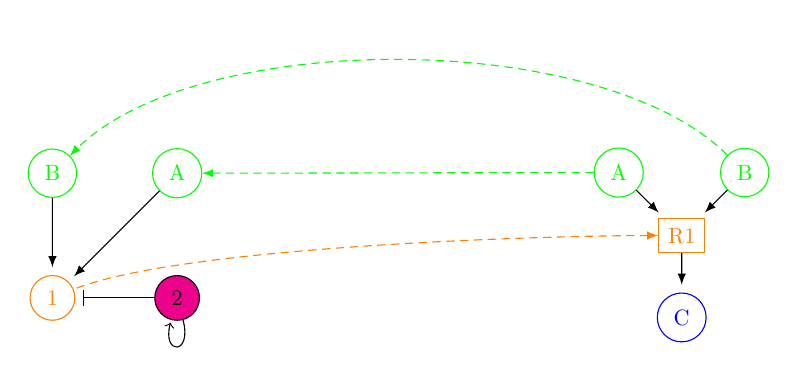
\begin{tikzpicture}[scale=0.8,transform shape]
  
  \node[draw,circle,inner sep=0.15cm,green] (A1) at (45:1.4cm) {A};
  \node[draw,circle,inner sep=0.15cm,green] (B1) at (135:1.4cm) {B};
  \node[draw,circle,inner sep=0.15cm,orange] (1) at (225:1.4cm) {1};
  \node[draw,circle,inner sep=0.15cm, fill=magenta] (2) at (315:1.4cm) {2};

  \node[draw,circle,inner sep=0.15cm,green] (A2) at (8cm,1cm) {A};
  \node[draw,circle,inner sep=0.15cm,green] (B2) at (10cm,1cm) {B};
  \node[draw,shape=rectangle,inner sep=0.15cm,orange] (R) at (9cm,0cm) {R1};
  \node[draw,circle,inner sep=0.15cm,blue] (C) at (9cm,-1.3cm) {C};

  \draw[shorten >=0.1cm,-latex] (A2) edge (R);
  \draw[shorten >=0.1cm,-latex] (B2) edge (R);
  \draw[shorten >=0.1cm,-latex] (R) edge (C);


  \path (A2) edge[-latex,green, out=180, in=0,densely dashed,looseness=0.5] (A1)
        (B2) edge[-latex,green, out=135, in=45,densely dashed,looseness=0.7] (B1)
        (R) edge[latex-,orange, out=180, in=22,densely dashed,looseness=0.5] (1);

  \draw[shorten >=0.1cm,-latex] (A1) edge (1);
  \draw[shorten >=0.1cm,-latex] (B1) edge (1);
  \draw[shorten >=0.1cm,-|] (2) edge (1);
  \draw[shorten >=0.1cm,-latex] (2) edge [loop below] (2);

\end{tikzpicture}

However, this solution keeps always at least one gene working. This means that this solution is worse than producing all the time the enzyme that catalyses the reaction
(the trivial solution). Another solution is shown below.

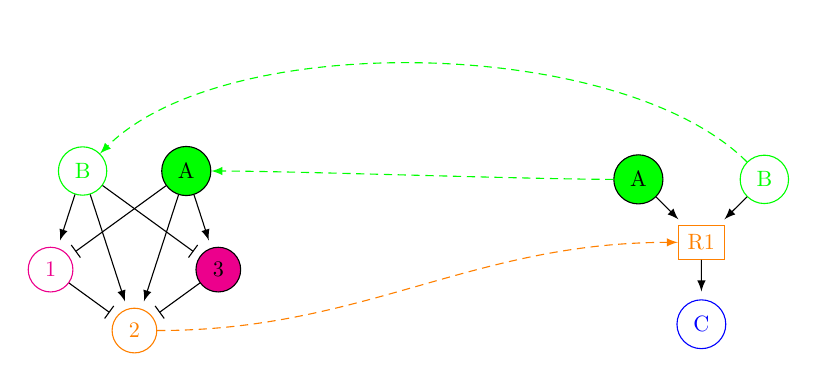
\begin{tikzpicture}[scale=0.8,transform shape]
  
  \node[draw,circle,inner sep=0.15cm,fill=green] (A1) at (54:1.4cm) {A};
  \node[draw,circle,inner sep=0.15cm,green] (B1) at (126:1.4cm) {B};
  \node[draw,circle,inner sep=0.15cm,magenta] (1) at (198:1.4cm) {1};
  \node[draw,circle,inner sep=0.15cm, orange] (2) at (270:1.4cm) {2};
  \node[draw,circle,inner sep=0.15cm, fill=magenta] (3) at (342:1.4cm) {3};

  \node[draw,circle,inner sep=0.15cm,fill=green] (A2) at (8cm,1cm) {A};
  \node[draw,circle,inner sep=0.15cm,green] (B2) at (10cm,1cm) {B};
  \node[draw,shape=rectangle,inner sep=0.15cm,orange] (R) at (9cm,0cm) {R1};
  \node[draw,circle,inner sep=0.15cm,blue] (C) at (9cm,-1.3cm) {C};

  \draw[shorten >=0.1cm,-latex] (A2) edge (R);
  \draw[shorten >=0.1cm,-latex] (B2) edge (R);
  \draw[shorten >=0.1cm,-latex] (R) edge (C);


  \path (A2) edge[-latex,green, out=180, in=0,densely dashed,looseness=0.5] (A1)
        (B2) edge[-latex,green, out=135, in=45,densely dashed,looseness=0.7] (B1)
        (R) edge[latex-,orange, out=180, in=0,densely dashed,looseness=1.0] (2);

  \draw[shorten >=0.1cm,-latex] (A1) edge (2);
  \draw[shorten >=0.1cm,-latex] (B1) edge (2);
  \draw[shorten >=0.1cm,-latex] (B1) edge (1);
  \draw[shorten >=0.1cm,-|] (B1) edge (3);
  \draw[shorten >=0.1cm,-|] (A1) edge (1);
  \draw[shorten >=0.1cm,-latex] (A1) edge (3);
  \draw[shorten >=0.1cm,-|] (1) edge (2);
  \draw[shorten >=0.1cm,-|] (3) edge (2);


\end{tikzpicture}

This solution is better and topologically more complicated, but still not good enough. It is better than the trivial solution, but less advantageous than 
responding to only one of the nutrients. It is important to mention that the fitness of an organism is not explicitly defined in this model. Organisms simply acccumulate 
biomass and divide whenever they reach a certain division threshold. These two examples have similar activation pattern for the enzyme but different division rates (and 
fitness). The best solution, fixing all the thresholds to zero, would be to produce the enzyme whenever one of the two nutrients - say $A$ - is present. In that case, the 
organism learns how to shut down its metabolism half of the time. But still, the enzyme is necessary only half of the time it is being produced.

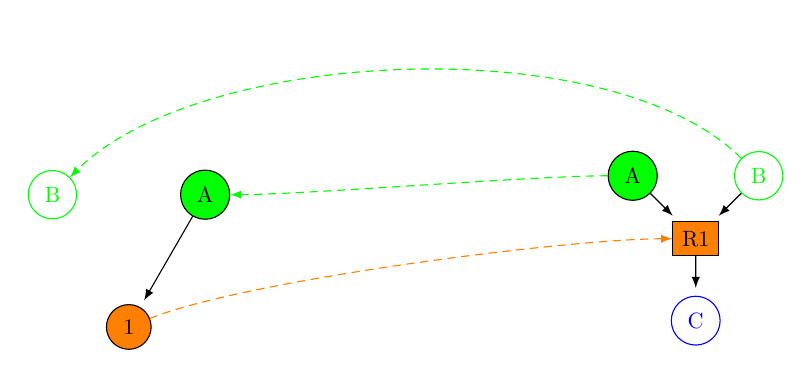
\begin{tikzpicture}[scale=0.8,transform shape]
  
  \node[draw,circle,inner sep=0.15cm,fill=green] (A1) at (30:1.4cm) {A};
  \node[draw,circle,inner sep=0.15cm,green] (B1) at (150:1.4cm) {B};
  \node[draw,circle,inner sep=0.15cm,fill=orange] (1) at (270:1.4cm) {1};

  \node[draw,circle,inner sep=0.15cm,fill=green] (A2) at (8cm,1cm) {A};
  \node[draw,circle,inner sep=0.15cm,green] (B2) at (10cm,1cm) {B};
  \node[draw,shape=rectangle,inner sep=0.15cm,fill=orange] (R) at (9cm,0cm) {R1};
  \node[draw,circle,inner sep=0.15cm,blue] (C) at (9cm,-1.3cm) {C};

  \draw[shorten >=0.1cm,-latex] (A2) edge (R);
  \draw[shorten >=0.1cm,-latex] (B2) edge (R);
  \draw[shorten >=0.1cm,-latex] (R) edge (C);


  \path (A2) edge[-latex,green, out=180, in=0,densely dashed,looseness=0.5] (A1)
        (B2) edge[-latex,green, out=135, in=45,densely dashed,looseness=0.7] (B1)
        (R) edge[latex-,orange, out=180, in=22,densely dashed,looseness=0.5] (1);

  \draw[shorten >=0.1cm,-latex] (A1) edge (1);


\end{tikzpicture}

That leads us to investigate the natural problem where each gene has a different threshold, and these thresholds are also subject to mutation. Doing that, learning 
becomes possible. The boolean network below only switches on the enzyme when both $A$ and $B$ are present, and no other genes are necessary to solve the task.

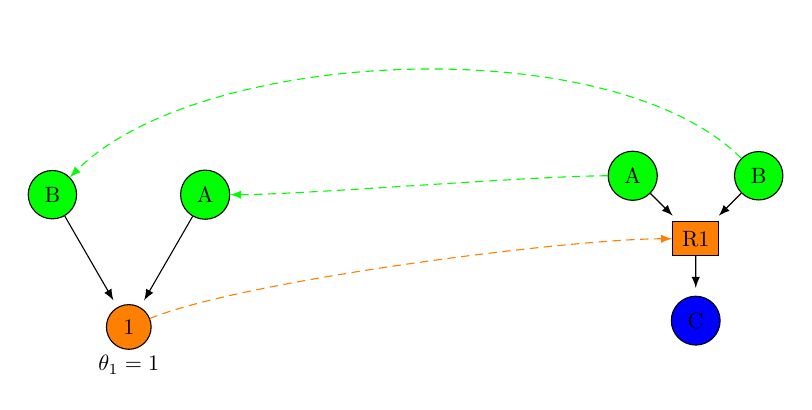
\begin{tikzpicture}[scale=0.8,transform shape]
  
  \node[draw,circle,inner sep=0.15cm,fill=green] (A1) at (30:1.4cm) {A};
  \node[draw,circle,inner sep=0.15cm,fill=green] (B1) at (150:1.4cm) {B};
  \node[draw,circle,inner sep=0.15cm,fill=orange] (1) at (270:1.4cm) {1};
  \node (label) at (270:2cm) {$\theta_1 = 1$};

  \node[draw,circle,inner sep=0.15cm,fill=green] (A2) at (8cm,1cm) {A};
  \node[draw,circle,inner sep=0.15cm,fill=green] (B2) at (10cm,1cm) {B};
  \node[draw,shape=rectangle,inner sep=0.15cm,fill=orange] (R) at (9cm,0cm) {R1};
  \node[draw,circle,inner sep=0.15cm,fill=blue] (C) at (9cm,-1.3cm) {C};

  \draw[shorten >=0.1cm,-latex] (A2) edge (R);
  \draw[shorten >=0.1cm,-latex] (B2) edge (R);
  \draw[shorten >=0.1cm,-latex] (R) edge (C);


  \path (A2) edge[-latex,green, out=180, in=0,densely dashed,looseness=0.5] (A1)
        (B2) edge[-latex,green, out=135, in=45,densely dashed,looseness=0.7] (B1)
        (R) edge[latex-,orange, out=180, in=22,densely dashed,looseness=0.5] (1);

  \draw[shorten >=0.1cm,-latex] (A1) edge (1);
  \draw[shorten >=0.1cm,-latex] (B1) edge (1);


\end{tikzpicture}

If we increase the number of educts, the same solution still holds. That justifies the use of varying thresholds. Now the problem becomes understanding how a 
population would behave inside of a landscape of an implicitly defined fitness. However, given an environmental pattern we can deduce average rates of production
of biomass and consequently derive the division rates associated to each genotype. For fixed threshold the genotype network looks like a Hamming graph like the one below 
for two sensor nodes and one gene. Otherwise, it is the cartesian product between this hamming graph and a path graph.


\begin{center}
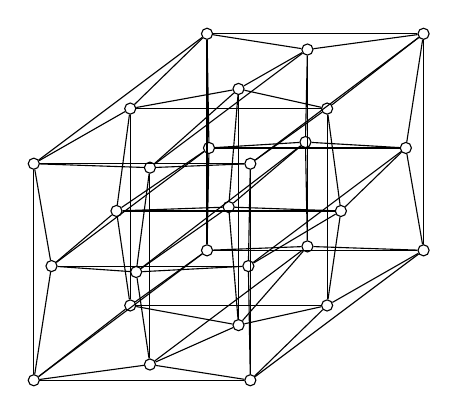
\begin{tikzpicture}[scale=0.25]

\node[draw,circle,inner sep=0.05cm] (0) at (-9.9,-8.8) {};   
\node[draw,circle,inner sep=0.05cm] (1) at (-4,-8) {};%
\node[draw,circle,inner sep=0.05cm] (2) at (1.1,-8.8) {};
\node[draw,circle,inner sep=0.05cm] (3) at (-5,-5) {};%
\node[draw,circle,inner sep=0.05cm] (4) at (0.5,-6) {};%%
\node[draw,circle,inner sep=0.05cm] (5) at (5,-5) {};%
\node[draw,circle,inner sep=0.05cm] (6) at (-1.1,-2.2) {};
\node[draw,circle,inner sep=0.05cm] (7) at (4,-2) {};%
\node[draw,circle,inner sep=0.05cm] (8) at (9.9,-2.2) {};
\node[draw,circle,inner sep=0.05cm] (9) at (-9,-3) {};%
\node[draw,circle,inner sep=0.05cm] (10) at (-4.7,-3.3) {};%%
\node[draw,circle,inner sep=0.05cm] (11) at (1,-3) {};%
\node[draw,circle,inner sep=0.05cm] (12) at (-5.7,-0.2) {};%%
\node[draw,circle,inner sep=0.05cm] (13) at (0,0) {};%                                       
\node[draw,circle,inner sep=0.05cm] (14) at (5.7,-0.2) {};%%                                       
\node[draw,circle,inner sep=0.05cm] (15) at (-1,3) {};%                                    
\node[draw,circle,inner sep=0.05cm] (16) at (3.9,3.3) {};%%
\node[draw,circle,inner sep=0.05cm] (17) at (9,3) {};%
\node[draw,circle,inner sep=0.05cm] (18) at (-9.9,2.2) {};
\node[draw,circle,inner sep=0.05cm] (19) at (-4,2) {};%
\node[draw,circle,inner sep=0.05cm] (20) at (1.1,2.2) {};
\node[draw,circle,inner sep=0.05cm] (21) at (-5,5) {};%
\node[draw,circle,inner sep=0.05cm] (22) at (0.5,6) {};%%
\node[draw,circle,inner sep=0.05cm] (23) at (5,5) {};%
\node[draw,circle,inner sep=0.05cm] (24) at (-1.1,8.8) {};
\node[draw,circle,inner sep=0.05cm] (25) at (4,8) {};%
\node[draw,circle,inner sep=0.05cm] (26) at (9.9,8.8) {};

\draw (0) edge (1);
\draw (1) edge (2);
\draw (2) edge (0);
\draw (3) edge (4);
\draw (4) edge (5);
\draw (5) edge (3);
\draw (6) edge (7);
\draw (7) edge (8);
\draw (8) edge (6);
\draw (9) edge (10);
\draw (10) edge (11);
\draw (11) edge (9);
\draw (12) edge (13);
\draw (13) edge (14);
\draw (14) edge (12);
\draw (15) edge (16);
\draw (16) edge (17);
\draw (17) edge (15);
\draw (18) edge (19);
\draw (19) edge (20);
\draw (20) edge (18);
\draw (21) edge (22);
\draw (22) edge (23);
\draw (23) edge (21);
\draw (24) edge (25);
\draw (25) edge (26);
\draw (26) edge (24);

\draw (0) edge (3);
\draw (3) edge (6);
\draw (6) edge (0);
\draw (1) edge (4);
\draw (4) edge (7);
\draw (7) edge (1);
\draw (2) edge (5);
\draw (5) edge (8);
\draw (8) edge (2);
\draw (9) edge (12);
\draw (12) edge (15);
\draw (15) edge (9);
\draw (10) edge (13);
\draw (13) edge (16);
\draw (16) edge (10);
\draw (11) edge (14);
\draw (14) edge (17);
\draw (17) edge (11);
\draw (18) edge (21);
\draw (21) edge (24);
\draw (24) edge (18);
\draw (19) edge (22);
\draw (22) edge (25);
\draw (25) edge (19);
\draw (20) edge (23);
\draw (23) edge (26);
\draw (26) edge (20);

\draw (0) edge (9);
\draw (9) edge (18);
\draw (18) edge (0);
\draw (1) edge (10);
\draw (10) edge (19);
\draw (19) edge (1);
\draw (2) edge (11);
\draw (11) edge (20);
\draw (20) edge (2);
\draw (3) edge (12);
\draw (12) edge (21);
\draw (21) edge (3);
\draw (4) edge (13);
\draw (13) edge (22);
\draw (22) edge (4);
\draw (5) edge (14);
\draw (14) edge (23);
\draw (23) edge (5);
\draw (6) edge (15);
\draw (15) edge (24);
\draw (24) edge (6);
\draw (7) edge (16);
\draw (16) edge (25);
\draw (25) edge (7);
\draw (8) edge (17);
\draw (17) edge (26);
\draw (26) edge (8);




\end{tikzpicture}
\end{center}

Given that, we are studying the behaviour of the population on top of this landscape depending on some parameters and conditions. We use thresholds varying from $-5$ to $4$. 
Then, we can gather all the genotypes into groups of phenotypes and explore how the innovations take place from one neutral network to another. The usual initial conditions
are like indicated below.


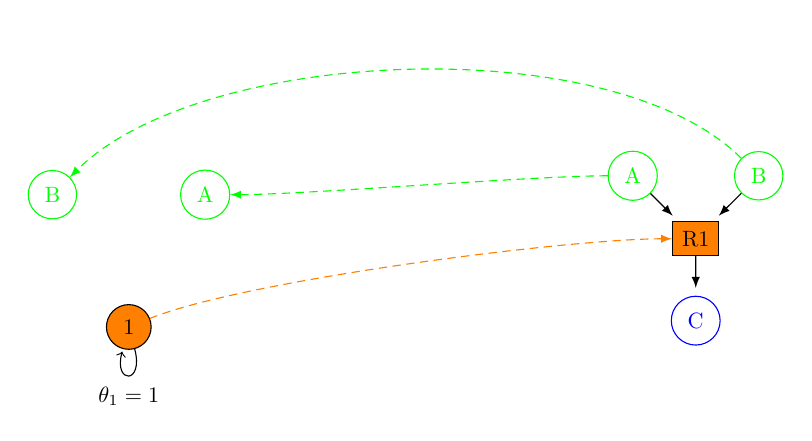
\begin{tikzpicture}[scale=0.8,transform shape]
  
  \node[draw,circle,inner sep=0.15cm,green] (A1) at (30:1.4cm) {A};
  \node[draw,circle,inner sep=0.15cm,green] (B1) at (150:1.4cm) {B};
  \node[draw,circle,inner sep=0.15cm,fill=orange] (1) at (270:1.4cm) {1};
  \node (label) at (270:2.5cm) {$\theta_1 = 1$};

  \node[draw,circle,inner sep=0.15cm,green] (A2) at (8cm,1cm) {A};
  \node[draw,circle,inner sep=0.15cm,green] (B2) at (10cm,1cm) {B};
  \node[draw,shape=rectangle,inner sep=0.15cm,fill=orange] (R) at (9cm,0cm) {R1};
  \node[draw,circle,inner sep=0.15cm,blue] (C) at (9cm,-1.3cm) {C};

  \draw[shorten >=0.1cm,-latex] (A2) edge (R);
  \draw[shorten >=0.1cm,-latex] (B2) edge (R);
  \draw[shorten >=0.1cm,-latex] (R) edge (C);


  \path (A2) edge[-latex,green, out=180, in=0,densely dashed,looseness=0.5] (A1)
        (B2) edge[-latex,green, out=135, in=45,densely dashed,looseness=0.7] (B1)
        (R) edge[latex-,orange, out=180, in=22,densely dashed,looseness=0.5] (1);

  \draw[shorten >=0.1cm,-latex] (1) edge [loop below] (1);


\end{tikzpicture}

It is possible to group, in this case, $270$ different genotypes into only $8$ different fitness classes. To our purposes, only four of them will matter. The first (and less 
fit) correspond to organisms that never produce the enzyme (SD). The second contains organisms that keep their gene always on (SL), and never interrupt the production 
of the enzyme, even if the chemical reaction is not possible. The third class (VL3) gathers genotypes that switch off partially when $A$ and $B$  are not present at the 
same time. And finally, the most fit which correspond to a single genotype that performs the AND function and switches off whenever unnecessary (VL4). We observe the 
relative amounts of the phenotypes in the population as a function of time. We compared both discrete stochastic simulations with a continuous linear approach. Both 
capture a transition to extinction and also the fact that, before the population finds the optimal solution it usually goes through an intermediate phenotype. 

\begin{figure}[hbtp]
 \begin{center}$
 \begin{array}{cc}
  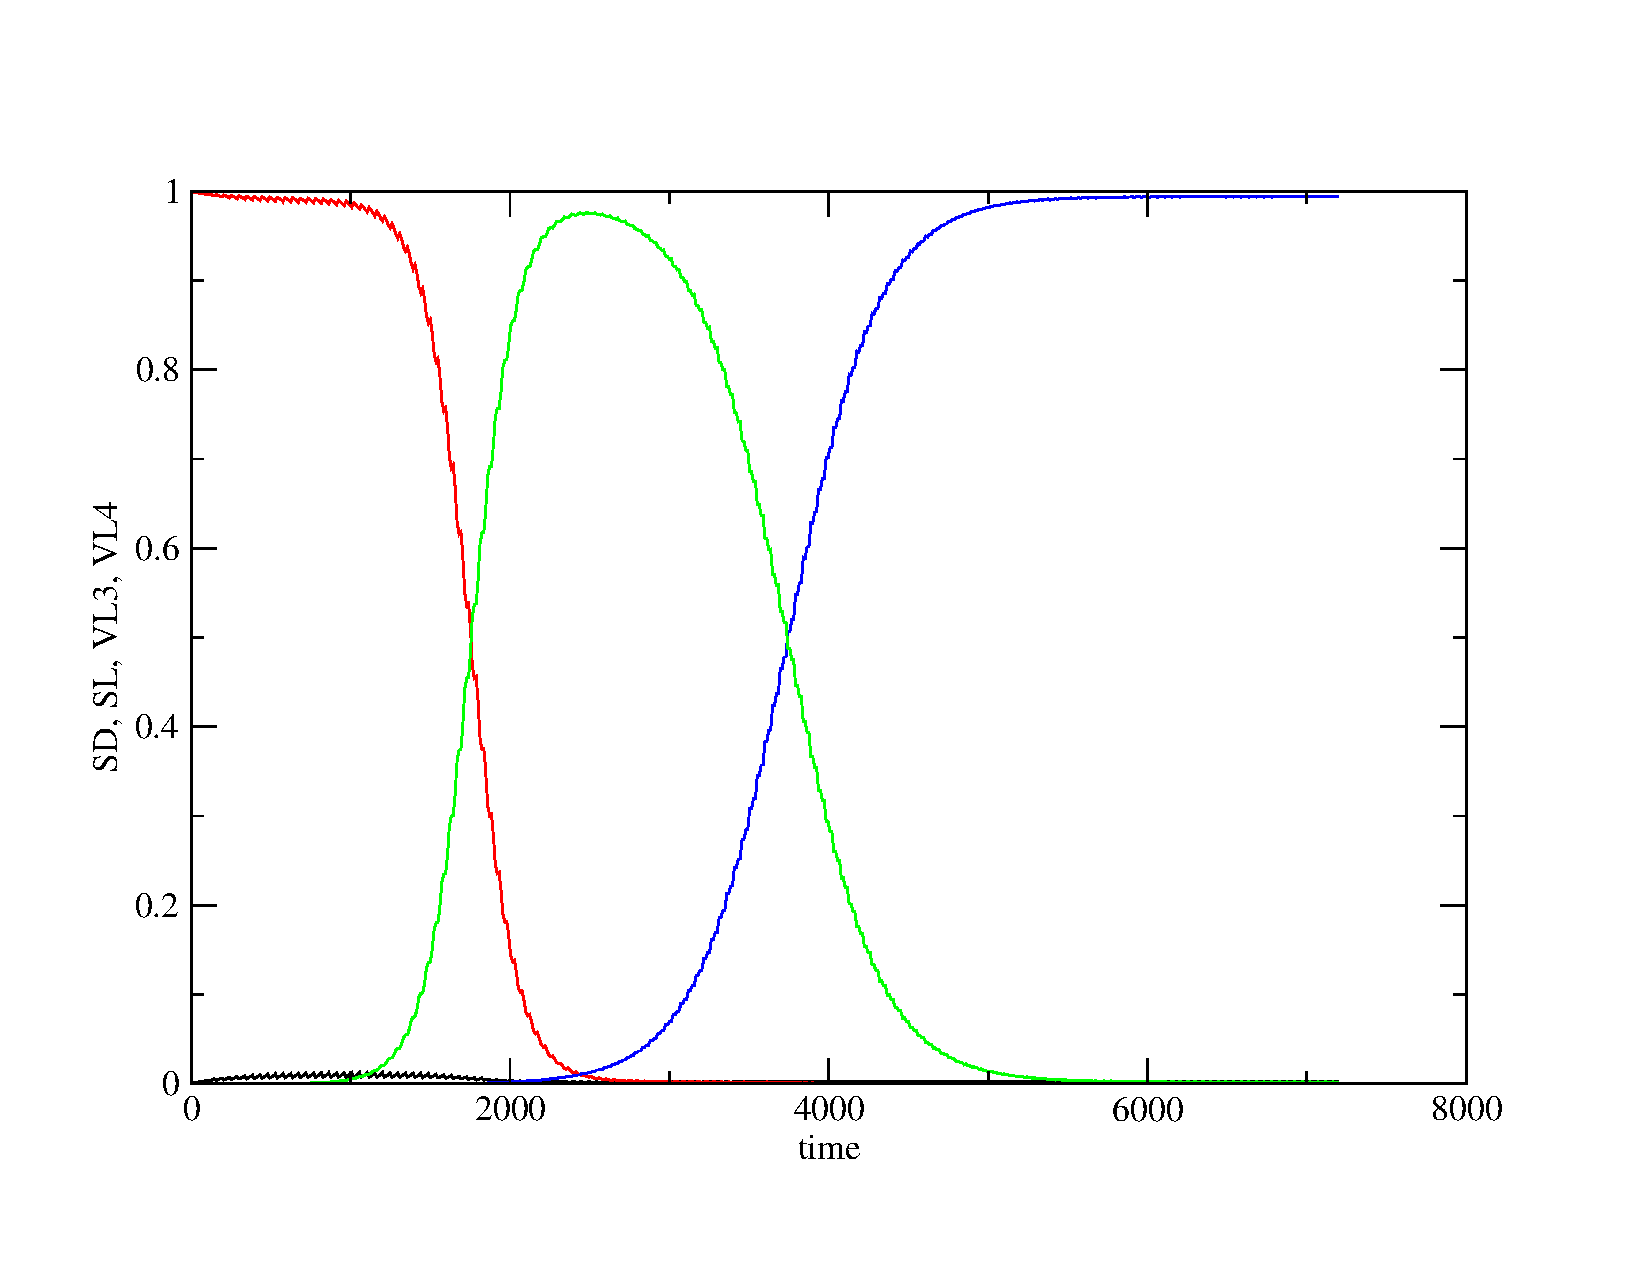
\includegraphics[keepaspectratio=true, width=5cm]{rho.pdf}&
  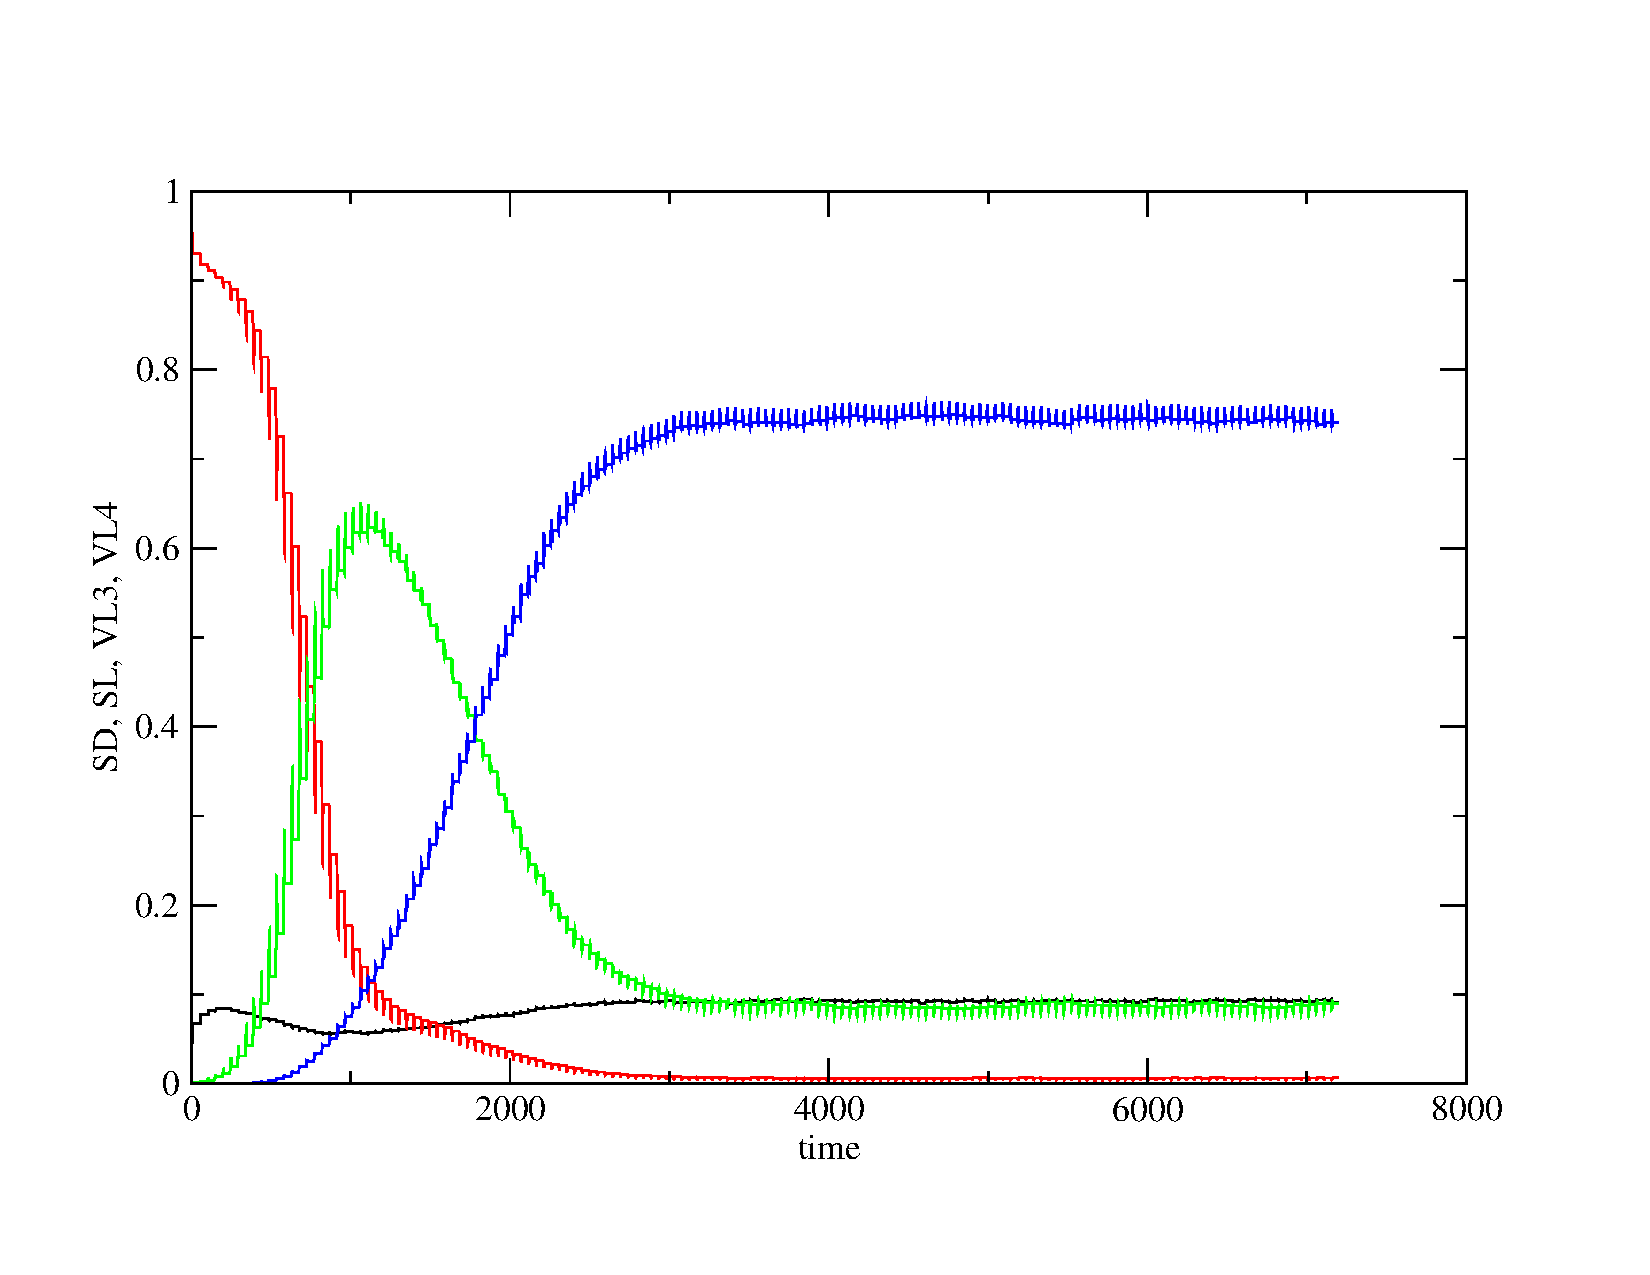
\includegraphics[keepaspectratio=true, width=5cm]{rhod.pdf}
\end{array}$
\caption{The first row shows the solution of the linear system given by the landscape, whereas the bottom row is an ensemble average of stochastic discrete simulations.}
  \end{center}

\end{figure}

The green curve corresponds to the VL3 intermediate population before the solution is found. For small mutation rates, the dynamics of the discrete case are governed by
rare events, abrupt transitions from one neutral network to the other.

Another important aspect to mention is that, if we increase the period where both nutrients are available, it is not anymore a big advantage to have such boolean 
networks, and the population unlearns this solution. This is captured by both discrete and continuous approaches. This is  what makes the definition of fitness subtle 
and not simple to deal with. Especially if one thinks of more complex patterns of availability of nutrients. This process is actually governing the evolution of the 
gene regulatory networks. Another counterintuitive result relates to the division mechanism of the population. We compared two different process - one involving 
generation overlap and the other without - and they have shown to be considerably different in respect to trajectories in configuration space and its attractors. 

We could see that different reproduction mechanisms lead to different attractor structures in the landscape, and increasing the size of the network will also
make the process much richer. The next steps go in the direction of increasing the size of both networks and understanding how the interaction between them 
will select topologies. Being a history-dependent process, evolution is a highly non-ergodic process and unraveling its mechanisms requires a more subtle understanding 
of out-of-equilibrium statistics. For future projects we intend to use a more detailed description of the metabolic network, involving reaction rates and concentrations 
of the metabolites, in an attempt to connect boolean networks and flux-balance analysis.



\end{document}

